% AP Statistics Video Follow-Along Worksheet
% Unit 3: Collecting Data | Lessons 6-7

\documentclass[11pt]{article}
\usepackage[margin=0.85in, headheight=14pt]{geometry}
\usepackage{enumitem}
\usepackage{amsmath}
\usepackage{amssymb}
\usepackage{fancyhdr}
\usepackage{tcolorbox}
\usepackage{array}
\usepackage{booktabs}
\usepackage{xcolor}
\usepackage{tikz}
\usetikzlibrary{shapes.geometric, arrows.meta, positioning}

% Define colors
\definecolor{apblue}{RGB}{0, 51, 102}
\definecolor{lightgray}{RGB}{245, 245, 245}
\definecolor{boxborder}{RGB}{180, 180, 180}

% Header setup
\pagestyle{fancy}
\fancyhf{}
\lhead{AP Statistics}
\chead{Unit 3: Collecting Data}
\rhead{Lessons 6--7}
\lfoot{Name: \underline{\hspace{2.5in}}}
\rfoot{Period: \underline{\hspace{0.75in}}}

% Custom box environments
\tcbset{
    vocabbox/.style={
        colback=lightgray,
        colframe=boxborder,
        boxrule=1pt,
        arc=3pt,
        left=8pt,
        right=8pt,
        top=6pt,
        bottom=6pt
    },
    objectivebox/.style={
        colback=white,
        colframe=apblue,
        boxrule=1.5pt,
        arc=3pt,
        left=8pt,
        right=8pt,
        top=6pt,
        bottom=6pt
    }
}

% Blank line command
\newcommand{\blank}[1]{\underline{\hspace{#1}}}

\begin{document}

% Title
\begin{center}
    {\Large \textbf{Topics 3.6--3.7: Selecting an Experimental Design \& Inference}}\\[4pt]
    {\large \textit{How do we choose and interpret well-designed experiments?}}\\[8pt]
    \textbf{Video Follow-Along Worksheet}
\end{center}

\vspace{0.5em}

% Learning Objective Box
\begin{tcolorbox}[objectivebox]
\textbf{Learning Objective (VAR-3.D):} Explain why a particular experimental design is appropriate.\\[4pt]
\textbf{Learning Objective (VAR-3.E):} Interpret the results of a well-designed experiment.\\[4pt]
\textbf{Essential Knowledge:} A randomized block design separates natural variability from treatment effects. Statistical inference allows us to attribute conclusions from sample data to the population. Statistically significant differences are evidence that treatments caused the observed effect.
\end{tcolorbox}

\vspace{0.5em}

% Vocabulary Box
\begin{tcolorbox}[vocabbox, title={\textbf{Key Vocabulary}}]
\begin{tabular}{@{}p{1.6in}p{4.3in}@{}}
\textbf{Randomized Block Design} & An experimental design where subjects are first grouped by a characteristic (block), then randomly assigned to treatments within each block \\[4pt]
\textbf{Matched Pairs Design} & A special case of blocking using pairs of similar experimental units, with one receiving each treatment \\[4pt]
\textbf{Blinding} & A technique where subjects and/or researchers are unaware of which treatment is being administered \\[4pt]
\textbf{Statistical Significance} & When observed differences between groups are too large to be reasonably attributed to chance alone \\[4pt]
\textbf{Statistical Inference} & Using sample data to draw conclusions about a population or treatment
\end{tabular}
\end{tcolorbox}

\vspace{1em}

%==============================================================================
% VIDEO 1: Topic 3.6 Daily Video 1 - Blocking & Blinding
%==============================================================================

\section*{Video 1: Blocking \& Blinding (Topic 3.6) \hfill \normalfont\small 5:54}

\subsection*{Part A: Introduction \& High Cholesterol Example \hfill \normalfont\small [0:00--0:53]}

\begin{enumerate}[label=\arabic*., leftmargin=2em]
    \item In this video, we will learn how \blank{1.25in} can improve the design of an experiment and under what conditions an experiment can be \blank{1.25in}.
    
    \vspace{0.5em}
    
    \item The ``High Cholesterol'' example is a \blank{1.75in} from a previous AP exam.
\end{enumerate}

\vspace{0.75em}

\subsection*{Part B: Completely Randomized Design \hfill \normalfont\small [0:53--2:29]}

\begin{enumerate}[label=\arabic*., leftmargin=2em, resume]
    \item A well-designed experiment includes four key components: \blank{1.5in} of treatments, \blank{1.5in}, replication, and \blank{1in}.
    
    \vspace{0.5em}
    
    \item To randomly assign 200 volunteers to two groups, we can number them 1 to 200, then use a \blank{1.75in} to select 100 numbers without repeat.
    
    \vspace{0.5em}
    
    \item The 100 randomly selected volunteers receive the \blank{1in} drug, and the remaining 100 receive the \blank{1in} drug.
    
    \vspace{0.5em}
    
    \item After treatment, we measure and compare the \blank{1.75in} for both groups.
\end{enumerate}

\vspace{0.75em}

% Diagram for completely randomized design
\begin{center}
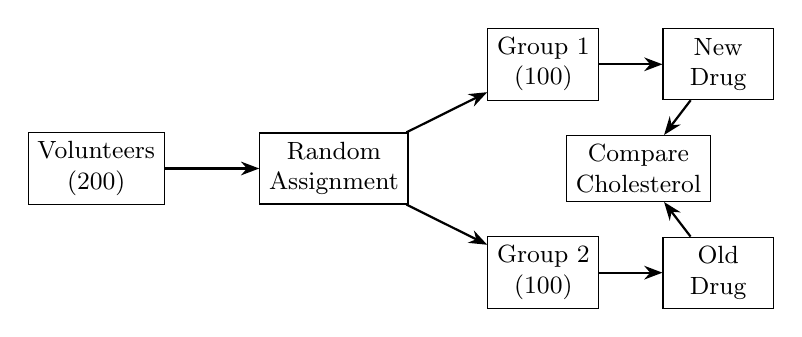
\begin{tikzpicture}[
    node distance=0.8cm and 1.2cm,
    box/.style={rectangle, draw, minimum width=1.4cm, minimum height=0.7cm, align=center, font=\small},
    arrow/.style={-{Stealth}, thick}
]
    \node[box] (vol) {Volunteers\\(200)};
    \node[box, right=of vol] (rand) {Random\\Assignment};
    \node[box, above right=0.4cm and 1cm of rand] (g1) {Group 1\\(100)};
    \node[box, below right=0.4cm and 1cm of rand] (g2) {Group 2\\(100)};
    \node[box, right=0.8cm of g1] (new) {New\\Drug};
    \node[box, right=0.8cm of g2] (old) {Old\\Drug};
    \node[box, right=2cm of rand, yshift=0cm] (comp) {Compare\\Cholesterol};
    
    \draw[arrow] (vol) -- (rand);
    \draw[arrow] (rand) -- (g1);
    \draw[arrow] (rand) -- (g2);
    \draw[arrow] (g1) -- (new);
    \draw[arrow] (g2) -- (old);
    \draw[arrow] (new) -- (comp);
    \draw[arrow] (old) -- (comp);
\end{tikzpicture}
\end{center}

\subsection*{Part C: Randomized Block Design \hfill \normalfont\small [2:51--4:16]}

\begin{enumerate}[label=\arabic*., leftmargin=2em, resume]
    \item From the prompt: ``High cholesterol level can be reduced by \blank{1.25in} \textit{or} by drug treatment.''
    
    \vspace{0.5em}
    
    \item This suggests that \blank{1.5in} could be a blocking variable that affects cholesterol levels.
    
    \vspace{0.5em}
    
    \item In a randomized block design, we first separate volunteers into \blank{1in} based on a characteristic (here: high vs.\ low exercise), \textit{then} perform randomization \blank{1.25in}.
    
    \vspace{0.5em}
    
    \item We then compare cholesterol levels \blank{1.5in} and overall.
\end{enumerate}

\vspace{0.5em}

% Diagram for randomized block design
\begin{center}
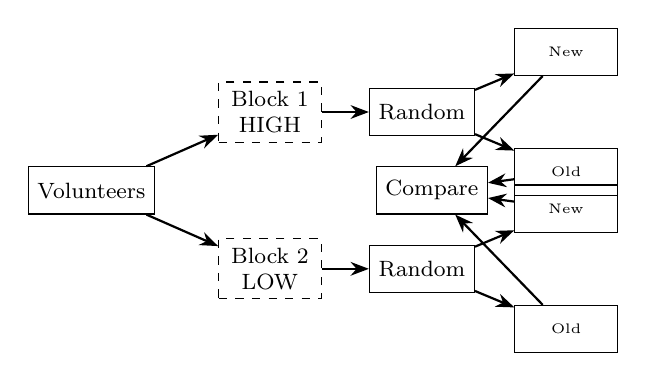
\begin{tikzpicture}[
    node distance=0.6cm and 0.9cm,
    box/.style={rectangle, draw, minimum width=1.3cm, minimum height=0.6cm, align=center, font=\footnotesize},
    block/.style={rectangle, draw, dashed, minimum width=1.3cm, minimum height=0.6cm, align=center, font=\footnotesize},
    arrow/.style={-{Stealth}, thick}
]
    \node[box] (vol) {Volunteers};
    
    % Blocking
    \node[block, above right=0.3cm and 0.8cm of vol] (b1) {Block 1\\HIGH};
    \node[block, below right=0.3cm and 0.8cm of vol] (b2) {Block 2\\LOW};
    
    % Random assignment within blocks
    \node[box, right=0.6cm of b1] (r1) {Random};
    \node[box, right=0.6cm of b2] (r2) {Random};
    
    % Treatments
    \node[box, above right=0.15cm and 0.5cm of r1, font=\tiny] (new1) {New};
    \node[box, below right=0.15cm and 0.5cm of r1, font=\tiny] (old1) {Old};
    \node[box, above right=0.15cm and 0.5cm of r2, font=\tiny] (new2) {New};
    \node[box, below right=0.15cm and 0.5cm of r2, font=\tiny] (old2) {Old};
    
    % Compare
    \node[box, right=2.8cm of vol] (comp) {Compare};
    
    \draw[arrow] (vol) -- (b1);
    \draw[arrow] (vol) -- (b2);
    \draw[arrow] (b1) -- (r1);
    \draw[arrow] (b2) -- (r2);
    \draw[arrow] (r1) -- (new1);
    \draw[arrow] (r1) -- (old1);
    \draw[arrow] (r2) -- (new2);
    \draw[arrow] (r2) -- (old2);
    \draw[arrow] (new1) -- (comp);
    \draw[arrow] (old1) -- (comp);
    \draw[arrow] (new2) -- (comp);
    \draw[arrow] (old2) -- (comp);
\end{tikzpicture}
\end{center}

\subsection*{Part D: Double Blinding \hfill \normalfont\small [4:16--5:27]}

\begin{enumerate}[label=\arabic*., leftmargin=2em, resume]
    \item If asked a yes/no question on the AP exam, make sure you answer \blank{1.25in} somewhere in your response.
    
    \vspace{0.5em}
    
    \item Double blinding is possible when both the \blank{1.25in} and the \blank{1.25in} are unaware of what treatments are being given to each subject.
    
    \vspace{0.5em}
    
    \item This works best if the treatments are similar in \blank{1in}, taste, or administration method.
\end{enumerate}

\vspace{0.75em}

\subsection*{Part E: Key Takeaways \hfill \normalfont\small [5:27--5:46]}

\begin{enumerate}[label=\arabic*., leftmargin=2em, resume]
    \item A randomized block design helps to separate \blank{1.75in} from differences due to the blocking variable.
    
    \vspace{0.5em}
    
    \item Blinding is possible when subjects and/or researchers are \blank{1.5in} of the treatment being administered.
\end{enumerate}

\vspace{1em}

%==============================================================================
% VIDEO 2: Topic 3.6 Daily Video 2 - Matched Pairs & Replication
%==============================================================================

\section*{Video 2: Matched Pairs \& Replication (Topic 3.6) \hfill \normalfont\small 6:48}

\subsection*{Part A: Tractor Plots Introduction \hfill \normalfont\small [0:00--1:22]}

\begin{enumerate}[label=\arabic*., leftmargin=2em, resume]
    \item This example is from the \blank{1.25in} AP exam (Form B).
    
    \vspace{0.5em}
    
    \item In this study, ``draft'' refers to the \blank{1.5in} needed to pull a plow.
    
    \vspace{0.5em}
    
    \item Identifying components of this experiment:
    \begin{itemize}[leftmargin=1.5em]
        \item Response variable: \blank{2in}
        \vspace{0.3em}
        \item Treatments: \blank{2.5in}
        \vspace{0.3em}
        \item Experimental units: \blank{2in}
    \end{itemize}
\end{enumerate}

\vspace{0.75em}

\subsection*{Part B: Evaluating Randomization \hfill \normalfont\small [2:10--2:41]}

\begin{enumerate}[label=\arabic*., leftmargin=2em, resume]
    \item Was randomization properly used? \blank{0.75in}
    
    \vspace{0.5em}
    
    \item Evidence: ``It was \blank{1.75in} which plot was to be plowed using the standard hitch.''
    
    \vspace{0.5em}
    
    \item The two \blank{1.25in} (treatments) were randomly assigned to the two \blank{1.25in} (experimental units).
\end{enumerate}

\vspace{0.75em}

\subsection*{Part C: Evaluating Replication \hfill \normalfont\small [3:09--4:02]}

\begin{enumerate}[label=\arabic*., leftmargin=2em, resume]
    \item Was replication properly used? \blank{0.75in}
    
    \vspace{0.5em}
    
    \item \textbf{Key insight:} Replication means applying each treatment to a sufficient number of \blank{1in}, not just taking multiple measurements.
    
    \vspace{0.5em}
    
    \item Problem: Each treatment was applied to only \blank{0.75in} experimental unit (plot). There were 25 measurements per plot, but this is \textit{not} replication.
\end{enumerate}

\vspace{0.75em}

\subsection*{Part D: Confounding Variable \hfill \normalfont\small [4:17--5:11]}

\begin{enumerate}[label=\arabic*., leftmargin=2em, resume]
    \item The draft is affected by environmental conditions such as \blank{0.9in}, terrain, and \blank{0.9in}.
    
    \vspace{0.5em}
    
    \item Because each hitch was used on only one plot, we cannot determine if the difference in draft is due to the \blank{1in} or the characteristics of that specific \blank{1in}.
    
    \vspace{0.5em}
    
    \item The treatments (hitches) are \blank{1.5in} with the plots.
\end{enumerate}

\vspace{0.75em}

\subsection*{Part E: Improving the Design \hfill \normalfont\small [5:11--6:20]}

\begin{enumerate}[label=\arabic*., leftmargin=2em, resume]
    \item \textbf{Improvement 1:} Split each plot in \blank{0.75in} and use random assignment to determine which hitch is used on either half. This reduces the \blank{1.5in} effect of the plot.
    
    \vspace{0.5em}
    
    \item \textbf{Improvement 2:} Use more than \blank{0.75in} experimental units.
    
    \vspace{0.5em}
    
    \item Don't forget to mention that you will measure the \blank{1.5in} after applying the treatments!
\end{enumerate}

\vspace{0.75em}

\subsection*{Part F: Key Takeaways \hfill \normalfont\small [6:20--6:48]}

\begin{enumerate}[label=\arabic*., leftmargin=2em, resume]
    \item Proper replication requires that multiple \blank{1.75in} receive the same treatment.
    
    \vspace{0.5em}
    
    \item A \blank{1.75in} design involves blocks of two similar experimental units, one receiving each treatment. \textit{OR} each experimental unit receives \blank{1in} treatments in random order.
\end{enumerate}

\newpage

%==============================================================================
% VIDEO 3: Topic 3.7 Daily Video 1 - Inference & Experiments
%==============================================================================

\section*{Video 3: Inference \& Experiments (Topic 3.7) \hfill \normalfont\small 5:50}

\subsection*{Part A: Introduction \& Learning Goals \hfill \normalfont\small [0:00--0:36]}

\begin{enumerate}[label=\arabic*., leftmargin=2em, resume]
    \item Three learning goals for this video:
    \begin{itemize}[leftmargin=1.5em]
        \item What is \blank{1.75in}?
        \vspace{0.3em}
        \item How does \blank{1.75in} help determine statistical significance?
        \vspace{0.3em}
        \item Under what conditions can results be \blank{1.5in} to the population?
    \end{itemize}
\end{enumerate}

\vspace{0.75em}

\subsection*{Part B: The R\'esum\'e Experiment \hfill \normalfont\small [0:36--2:19]}

\begin{enumerate}[label=\arabic*., leftmargin=2em, resume]
    \item In this study, two r\'esum\'es were identical except for the \blank{1in} (Greg Baker vs.\ Jamal Jones).
    
    \vspace{0.5em}
    
    \item R\'esum\'es were sent to employers in \blank{1.25in} and \blank{1.25in}.
    
    \vspace{0.5em}
    
    \item Each employer was \blank{1.5in} a r\'esum\'e with either a commonly White name or commonly African-American name.
    
    \vspace{0.5em}
    
    \item Check if this is a well-designed experiment:
    \begin{itemize}[leftmargin=1.5em]
        \item Comparison? \blank{0.5in} --- Two groups (White vs.\ African-American names)
        \vspace{0.2em}
        \item Random assignment? \blank{0.5in} --- Each company given a random name
        \vspace{0.2em}
        \item Replication? \blank{0.5in} --- \blank{1in} r\'esum\'es for each group
        \vspace{0.2em}
        \item Control? \blank{0.5in} --- All r\'esum\'es equal except for name
    \end{itemize}
\end{enumerate}

\vspace{0.75em}

\subsection*{Part C: Results of the R\'esum\'e Experiment \hfill \normalfont\small [2:19--3:00]}

\begin{enumerate}[label=\arabic*., leftmargin=2em, resume]
    \item Callback rate for r\'esum\'es with White names: \blank{1in}\%
    
    \vspace{0.5em}
    
    \item Callback rate for r\'esum\'es with African-American names: \blank{1in}\%
    
    \vspace{0.5em}
    
    \item Difference between groups: \blank{1in}\%
    
    \vspace{0.5em}
    
    \item The key question: Is this difference due to \blank{0.7in} alone, or is it because of the \blank{1in}?
\end{enumerate}

\vspace{0.75em}

\subsection*{Part D: Statistical Significance \hfill \normalfont\small [3:00--4:44]}

\begin{enumerate}[label=\arabic*., leftmargin=2em, resume]
    \item Random assignment allows us to conclude that very large observed changes are not merely by \blank{1in} (statistically significant).
    
    \vspace{0.5em}
    
    \item Statistically significant differences between treatment groups are evidence that the \blank{1.1in} caused the effect.
    
    \vspace{0.5em}
    
    \item Two possibilities for the 3.38\% difference:
    \begin{itemize}[leftmargin=1.5em]
        \item Option 1: Type of name does \textit{not} affect callback rate; the difference happened by \blank{1in}
        \item Option 2: Type of name \blank{1.25in} callback rate
    \end{itemize}
    
    \vspace{0.5em}
    
    \item The probability of observing an outcome this extreme due to chance was $p \approx$ \blank{1in}.
    
    \vspace{0.5em}
    
    \item Conclusion: We have \blank{2in} evidence that the type of name on a r\'esum\'e affects the likelihood of a callback.
\end{enumerate}

\vspace{0.75em}

\subsection*{Part E: Statistical Inference \& Generalization \hfill \normalfont\small [4:44--5:23]}

\begin{enumerate}[label=\arabic*., leftmargin=2em, resume]
    \item Statistical inference: Decisions from the \blank{1in} can be attributed to the \blank{1.25in} from which the sample was drawn.
    
    \vspace{0.5em}
    
    \item If experimental units are \blank{1.75in} of the population, then results can be generalized to the population.
    
    \vspace{0.5em}
    
    \item \blank{1.75in} of individuals gives a better chance that the sample will be representative.
\end{enumerate}

\vspace{0.75em}

\subsection*{Part F: Key Takeaways \hfill \normalfont\small [5:23--5:50]}

\begin{enumerate}[label=\arabic*., leftmargin=2em, resume]
    \item Statistical inference allows us to make \blank{1.25in} about populations or treatments based on sample data.
    
    \vspace{0.5em}
    
    \item Observed changes larger than can be attributed to chance are considered \blank{1.75in}.
    
    \vspace{0.5em}
    
    \item \blank{1.75in} of experimental units allows results to be generalized to the population of interest.
\end{enumerate}

\vspace{1em}

%==============================================================================
% POST-VIDEO REFLECTION
%==============================================================================

\section*{Post-Video Reflection}

\begin{enumerate}[label=\arabic*., leftmargin=2em, resume]
    \item \textbf{Random Selection vs.\ Random Assignment:} Explain the difference and when each is used.
    
    \vspace{1in}
    
    \item \textbf{Evaluating an Experiment:} A researcher wants to test whether a new fertilizer increases crop yield. She has 10 fields available, each with different soil types. She applies the new fertilizer to 5 fields and the old fertilizer to 5 fields, then measures yield.
    
    \begin{enumerate}[label=(\alph*)]
        \item What is a potential confounding variable in this study?
        
        \vspace{0.6in}
        
        \item Propose an improved design using blocking.
        
        \vspace{0.8in}
    \end{enumerate}
    
    \item \textbf{Interpreting Statistical Significance:} In a study comparing two medications, researchers found a statistically significant difference in recovery times ($p = 0.02$). What does this mean, and what can we conclude about causation?
    
    \vspace{1in}
    
    \item \textbf{Generalization:} Under what two conditions can the results of an experiment be generalized to a larger population?
    
    \vspace{0.8in}
\end{enumerate}

\vspace{0.5em}

%==============================================================================
% EXIT TICKET
%==============================================================================

\begin{tcolorbox}[colback=lightgray, colframe=apblue, boxrule=1.5pt, title={\textbf{Exit Ticket}}]
In 2--3 sentences, explain the relationship between random assignment, statistical significance, and establishing causation in experiments.

\vspace{1in}
\end{tcolorbox}

\end{document}
